The content of this chapter are primarily taken from ``Upper Limits on the Rates of Binary Neutron Star and Neutron-Star–Black-Hole Mergers from Advanced LIGO’S First Observing Run" in 2016. The main focus is on the results from the PyCBC offline search analysis conducted in this study.

Between September $12^\mathrm{th}$, $2015$ and January $19^\mathrm{th}$, $2016$, the two aLIGO detectors in Hanford, Washington and Livingston, Lousiana conducted their first observing period. During the first observing run two binary black hole coalescences were confidently observed by the offline PyCBC gravitational wave search pipeline with a p-value of being generated by noise of less than $10^{-7}$. A third candidate, termed LVT151012, was also observed by PyCBC, although with a smaller p-value. The masses of these binaries were assessed to not be compatible with the expected masses of neutron stars, and thus must be black hole binaries. This study assessed upper limits on the expected rate of mergers of neutron star binaries and neutron-star-black-hole binaries.

\section{The PyCBC Offline Search in the First Observing Run}
Below we briefly describe the methodology of the PyCBC Offline Search Pipeline in the first observing period.

The PyCBC Offline search analysis (cite) is a matched filter search for compact binary coalescence...

Derive matched-filter-snr...

\subsection{A Compact Binary Coalescence Template Bank}

The PyCBC Offline search is a modeled-search for gravitational waves from compact binary coalescence. And so we construct a bank of potential templates for astrophysical gravitational wave signals. This bank is referred to as the template bank and holds a catalog of gravitational wave signals that could be discovered. To do so we are required to generate templates in such a way as to span the parameter space of potential signals. In the first observing run, the template bank was a four-dimensional (parameter) bank. The four parameters were component masses of the binaries, $m_1$, $m_2$, and the component angular-momentum aligned-spin of the binary $\chi^z_1$ and $\chi^z_2$. The masses are drawn such that $m_1 > m_2$, which helps reduce the size of the template bank. The aligned-spin components are drawn to reflect the expected astrophysical properties of the binaries in that respective region of the mass parameter space.

The template bank is segmented into three sections, intended to find BNS, NSBH, and BBH signals. 
The template bnak in the first observing run consisted of approximately $250,000$ templates.

For $n$ detectors the harmonic mean of the detector's power spectral densities is chosen as the reference power spectral density when designing a common template bank for the Hanford and Livingston detectors. Previous searches used independent template banks for independent detectors, however this was not done in the first-observing run.

As the run progresses the template bank is validated using injected software signals to ensure that the noise properties of the detector have not changed to a sufficient degree as to make the template bank and template placement ineffectual in recovering expected signals. To do so, a population of simulated signals are expected to have a minimal match of $97 \%$ with any particular template in the bank. This is often called the Fitting Factor of the template bank. It is often a desired trait that less than $1\%$ of the simulated signals exhibit less than a $3 \%$ loss in anticipated signal-to-noise-ratio due to the discreteness of the template bank (or the change in the detector's power spectral density). The template bank was validated several times across the entire first observing run and only one template bank was necessary for the duration of the analysis.

\subsection{Data Quality and Conditioning}
It is well-known in the gravitational wave community that the output of the detector is not Gaussian and non-stationary over long periods of times and that the quality of the data from the interferometers is not always suitable for gravitational-wave analysis (cite). For this reason, the data undergo data quality checks and data conditioning prior to being analyzed for gravitational wave events.

In particular, there are several data quality vetoes

Gating

\subsection{The Ranking Statistic: Signal-to-Noise-Ratio and NewSNR}
Derive SNR from Gaussian distribution

Maximize over amplitude

Maximize over phase

However, the noise in the detector is decidedly not Gaussian, nor stationary and so the a new ranking statistic was developed as a further signal consistency check. The signal-to-noise-ratio statistic was made subject to a reduced $\chi^2$ consistency check, hence labeled as $\chi_r^2$. The $\chi_r^2$ test separates the signal into $k$ frequency bins and measures the accumulated signal-to-noise-ratio in each frequency bin. For a true signal, we expect a steady contribution to the signal-to-noise-ratio from each frequency bin. Thus, the $\chi_r^2$ test for a true signal embedded in Gaussian noise returns a value $\leq 1$, while a $\chi_r^2$ value $>1$ indicates a poor fit to the data across all frequency bins. The $\chi_r^2$ test can be expressed as:
\begin{equation}\label{eqn:reduced_chi_sq}
    \chi^2_r = \frac{k}{2k-2} \sum^k_{i=1} \left(\rho_i - \frac{\rho_i}{k}\right)^2
\end{equation}
Here $\rho_i$ represents the signal-to-noise-ratio in the $i^{\mathrm{th}}$ frequency bin, and $k$ is the number of frequency bins.

Prior to the first observing run, $k=16$ frequency bins were used, however, in the first observing run the number of frequency bins used was dependent on the peak frequency of the template. The formulation in the first observing run was, $k = 0.4\left[f_\mathrm{peak} / \mathrm{Hz}\right]^{2/3}$, and $k$ is rounded to the nearest integer. Next, the reduced $chi^2$ values are used to re-rank the signal-to-noise-ratio ranking statistic through an empirically designed ranking statistic called newSNR. When $\chi^2_r > 1$, newSNR can be calculated as:
\begin{equation}\label{eqn:newsnr}
    \hat{\rho} = \frac{\rho}
                  {\left\{\left[ 1 + \left(\chi^2_r\right)^3\right]/2\right\}^{1/6}}
\end{equation}
For values of $\chi^2_r \leq 1$, NewSNR is equal to the signal-to-noise-ratio ($\hat{\rho} = \rho$), while for values of $\chi^2_r >1$, Eq.~\ref{eqn:newsnr} is applied and newSNR is less than the signal-to-noise-ratio ($\hat{\rho}_c < \rho$). Finally then, for the Livingston and Hanford detectors the ranking statistic of a candidate trigger is $\hat{\rho}^2_\mathrm{network} = \hat{\rho}_\mathrm{L1}^2 + \hat{\rho}_\mathrm{H1}^2$. For a more detailed description of the first observing run's ranking statistics and the $\chi^2_r$ please consult N, N.

\subsection{Evaluation of the Statistical Significance of Events}
Description of timeslides

After coincident triggers are collected across five days of coincident analysis time between the two detectors. These coincident triggers are the foreground event triggers and are potentially of astrophysical origin. In order to assess the statistical significance of these foreground triggers we need an estimate of the rate at which non-astrophysical or background noise could potentially generate triggers of similar magnitude in the ranking statistic. Unfortunately, gravitational waves cannot be shielded from as electromagnetic waves can be, and so we use an empirical method to estimate the false alarm rate of triggers at a specific loudness in ranking statistic.

Description of inclusive and exclusive background

Description of p-value evaluation for single events

Since $n=3$ independent PyCBC offline searches were carried out in the first observing run for different compact binary coalescences, a Bonferroni correction is applied to the measured p-values from each search. The Bonferroni correction, or trials factor, states that if one conducts $n$ trials in searching for an effect, the threshold $\alpha$ on the p-value should also be divided by the number of trials $n$. This provides a conservative method for re-ranking the statistical significance of events provided multiple instances of searches. Since the different CBC search categories are weakly correlated (e.g. GW150914 was seen in the BBH search and the BBH-NSBH search), a better p-value correction could be considered to be less than $3$. Quantifying this level of correlation however, was beyond the scope of the study.

The p-value of a particular event can then be converted to a z-score, or the number of standard deviations in a one-tailed Gaussian probability integral via: 
\begin{equation}
    z = - \sqrt{2} \, \mathrm{erf}^{-1} \left[1 -  2 \left(1-\, p\right)\right].
\end{equation}
Here $z$ represents the z-score, $\mathrm{erf}^{-1}$ is the inverse error function, and $p$ is shorthand for the p-value (e.g. $0.05$). It is standard practice in many subfields of physics to require a z-score of $5$ (sometimes called $5 \sigma$) level of confidence before rejecting the null hypothesis that noise generated the gravitational wave signals. This corresponds to a p-value of $< 10^{-7}$.

Additional data quality checks are then used to verify that the gravitational wave candidate is more consistent with a signal hypothesis than with the null (noise) hypothesis. The probability that the event is of astrophysical origin cannot be gathered from the p-value itself but requires the use of Bayes Rule to calculate the probability of being of astrophysical origin, $p_\mathrm{astro}$. P-values are statements about the probability of observing data greater than some critical value under the assumption that the null hypothesis is true, while the probability of the event being astrophysical is a probability of a hypothesis being true (that the signal model better \textit{explains} the candidate than a noise model).

\subsection{Results of the Search}


The PyCBC offline search analysis found two confident gravitational wave events, GW150914 and GW151226, with statistical significance $> 5 \sigma$ (p-value $<  10^{-7}$) and a gravitational wave candidate, LVT151012, with a statistical significance of $\sim 2\sigma$. These statistical significance values are quoted after a trials factor of $3$ was applied to the analysis. All three triggers were found to be consistent with stellar mass black hole binaries, although LVT151012 was not confidently claimed as a detection.

No statistically significant BNS or NSBH events were found. And so we turn towards trying to determine an upper limit on the rate of mergers of BNS and NSBH events.

\section{Bayesian Rates Estimation}
Since no events were discovered in the first observing run, we seek to try to model the expected number of events for BNS and NSBH events. The expected number of events $\Lambda$ can be expressed as:
\begin{equation}
    \Lambda = R \, \langle VT\rangle.
\end{equation}
Here, the rate of mergers is given by $R$, and $\langle VT\rangle$ describes the sensitive-spacetime volume averaged over space, observation time, and the parameters of the source population of interest. The units of a rate are henceforth in $\mathrm{Gpc}^{-3} \mathrm{yr}^{-1}$. For reference the core-collapse supernova rate is $\sim 10^5 \, \mathrm{Gpc}^{-3} \, \mathrm{yr}^{-1}$ (Cappellaro et al. 2015).

Here we assume that gravitational wave events are exceedingly rare, and so we can model the likelihood for finding an observation of a gravitational wave event in the data $D$ as a Poisson distribution. The likelihood of seeing $s_i$ independent events after $N$ observations, given some $\Lambda$ can be expressed as:
\begin{equation}\label{eqn:poisson_likelihood}
    p\left(s|\Lambda\right) = \prod_{i=1}^N \frac{1}{s_i!}\Lambda^{s_i} e^{-\Lambda}
\end{equation}
In the case that we have zero observations, in one observing period, this likelihood can be written as:
\begin{equation}\label{eqn:no_event_poiss_like}
    p\left(s|\Lambda\right) = e^{-\Lambda}.
\end{equation}
Using Bayes theorem we can find a posterior probability on the number of expected rates as:
\begin{equation}\label{eqn:posterior_lambda_simple}
    p\left(\Lambda|s\right) \propto p\left(\Lambda\right) p\left(s|\Lambda\right).
\end{equation}
Here $p\left(\Lambda\right)$ is our prior belief on $\Lambda$, the number of expected mergers. The most straightforward prior distribution to use is a conjugate prior distribution. The advantage of a conjugate prior distribution is that our posterior distribution will be of the same kind or type of distribution as the prior distribution. For a Poisson likelihood the conjugate prior is proportional to a Gamma probability distribution, in our case we express this as:
\begin{equation}\label{eqn:prior_lambda_simple}
    p\left(\Lambda\right) \propto \Lambda^{\alpha}.
\end{equation}
A conjugate prior when multiplied with its respective likelihood distribution gives a posterior distribution that is within the same family of functions as the prior distribution. Setting $\alpha=0$ gives a uniform prior distribution, while setting $\alpha = 1/2$ gives $p\left(\Lambda\right) \propto 1/\sqrt{\Lambda}$. This is the Jeffreys prior for the Poisson likelihood in that it is an uninformative prior. A Jeffreys prior is sometimes useful in that it gives a equal prior probability weight to all possible values of the parametrization of the Bayesian inference.

Prior information from previous LIGO data were not used in a prior on $\Lambda$ due to changes in the detector sensitivity and the large changes to $\langle VT\rangle$.

The likelihood $e^{-\Lambda}$ is estimated by empirically measuring $\langle VT\rangle$ through the use of software injections of gravitational wave events into the aLIGO data set. These software injections involve generating gravitational wave strain data for different astrophysical objects in the radiation frame and then projecting them into the detector frame. These simulated signals are then added in to aLIGO data for detection.

Simulated signals are considered to be recovered when they are detected with an IFAR of $> \, 100 \, yrs$.  Since only a finite set of software injections can be processed and recovered, we use Monte-Carlo integration techniques to estimate the volume of injections recovered and a variance estimate of the volume recovered. The volume of injections recovered is compared then to the spacetime volume that the injections were injected from. Furthermore, the uncertainty in the calibration of the detector plays a role in the uncertainty in the recovered volume, since the calibration of the data plays a role in recovered signal-to-noise-ratios of simulated signals. It was found that the calibration added an $18 \%$ uncertainty to the estimated sensitive volume $\langle VT \rangle$. There is an additional uncertainty due to waveform modelling between injected simulated signals and waveform models used for recovery. This is additionally folded into the uncertainty on $\langle VT \rangle$.

It is convenient to consider the posterior on $\Lambda$ as a joint-posterior on the variables that compose $\Lambda$, that being $R$ and $VT$. To do so we can refactor the prior distribution on $\Lambda$ into a joint prior distribution on $R$ and $\langle VT \rangle$.
\begin{equation}\label{eqn:joint_posterior_simple}
    p\left(R, \langle VT \rangle \right) = p\left(R | \langle VT \rangle\right) \, p\left( \langle VT \rangle \right).
\end{equation}
In this publication, the prior $p\left(R | \langle VT \rangle\right)$ was chosen to be uniform in $R$, or a Jeffreys prior given by, $1/\sqrt{R \langle VT \rangle}$. In keeping with previous Refs, (Abbott et al. 2016f,m,c), the prior distribution on $\langle VT \rangle$ is given as a log-normal distribution given by:
\begin{equation}\label{eqn:prior_vt}
    p\left(\langle VT \rangle \right) =
            ln \, \mathcal{N} \left( \mu, \sigma^2\right).
\end{equation}
Here $\mu$ is the average value for $\langle VT \rangle$ obtained from the offline search, and $\sigma$ represents the $18 \%$ uncertainty in $\langle VT \rangle$ due to calibration uncertainty.

Thus the posterior of $\Lambda$ in the new parametrization becomes:
\begin{equation}\label{eqn:posterior_lambda}
    p \left(R, \langle VT \rangle \right) \propto p\left(R, \langle VT \rangle \right) \, e^{-R \langle VT \rangle}.
\end{equation}
To obtain a posterior distribution on the rate $R$ of mergers of a certain class we are required to marginalize the joint-posterior in $R$ and $\langle VT \rangle$ over $\langle VT \rangle$. This can be expressed as:
\begin{equation}\label{eqn:posterior_rate}
    p\left(R | s\right) = \int p \left(R, \langle VT \rangle | s \right) d\langle VT \rangle.
\end{equation}
Finally then, the upper limit on the rate at the $90 \%$ credible level is possible by integrating the marginalized posterior distribution of $R$ from $0$ to an upper-value of $R_\mathrm{critical}$ that grants a $90 \%$ probability.
\begin{equation}\label{eqn:90perc_conf_int}
    0.9 = \int_0^{R_{\mathrm{critical}}} p\left(R | s\right) dR.
\end{equation}
For a uniform prior in $p \left(R, \langle VT \rangle | s \right)$ and no uncertainty in $\langle VT \rangle$ the $90 \%$ credible limit is given as:
\begin{equation}\label{eqn:freq_90_perc}
    R_{\mathrm{critical}} = \frac{- ln \left( 1 - 0.9 \right)}{\langle VT \rangle} = \frac{2.303}{\langle VT \rangle}.
\end{equation}
The expression in Eq.~\ref{eqn:freq_90_perc} is also the Frequentist's $90 \%$ confidence interval(cite Jolien), although one should be careful in that the interpretation of the intervals are distinct in Frequentism and Bayesianism. Under the Jeffreys prior on $p \left(R, \langle VT \rangle | s \right)$ the upper limit can be expressed as:
\begin{equation}\label{eqn:jeffreys_90_perc}
    R_{\mathrm{critical}} = \frac{\left[\mathrm{erf}^{-1}\left(0.9 \right) \right]^2}{\langle VT \rangle} = \frac{1.353}{\langle VT \rangle}.
\end{equation}

Using these expressions, we can thus model the rate of mergers $R$ of a particular class of binaries by conducting software injections for that class of binaries that model our expectations of the astrophysical population for that binary.

\subsection{Astrophysical Populations of BNS and NSBH}
There are thousands of identified neutron stars, of which the majority are detected as pulsars (). Of these there are an estimated 70 neutron stars identified as binary neutron stars. Mass estimates of neutron stars range between $\approx \, 1 M_\odot$ to $3 M_\odot$. Eight candidate neutron star binaries permitted measurement of the binary component masses (), of which an estimate of the distribution of events is consistent with $\mathcal{N} \left(\mu = 1.35, \sigma^2 = 0.13^2 \right)$.

With respect to the spin characteristics of neutron stars, the fastest spinning pulsar was measured to have a rotational frequency of $716 \, Hz$. For reasonable estimates of the mass and moment of inertia for this pulsar, this corresponds to a dimensionless spin $\chi = c |S| / (G m^2) \sim 0.4$, where $m$ is the mass of the pulsar, $c$ is the speed of light, $G$ is Newton's gravitational constant, and $|S|$ is the angular momentum. However, the fastest spinning neutron star in a binary system is estimated to have a $\chi \leq 0.04$ (Brown et al). A neutron star in a binary can be spun up to larger rotational frequencies if its binary companion accretes matter and angular momentum on to the neutron star. This is called a recycled neutron star and estimates of the spin of a possible candidate BNS pulsar J1807-2500B is $\chi \sim 0.2$.

With these things in mind, our simulated astrophysical population for neutron star binaries contains two distinct populations in the mass parameters that we simulate. The first BNS population is drawn uniform in component masses between $\left[1, 3\right] M_\odot$, while another population is drawn with mass distribution, $\mathcal{N} \left(\mu = 1.35, \sigma^2 = 0.13^2 \right)$. Each mass distribution is also subject to two distinct component spin distributions. The first spin distribution is an isotropic component-spin distribution such that $|\chi_i| < 0.05$. The second spin distribution is an isotropic component-spin distribution with $|\chi| < 0.4$. This second spin distribution is drawn with considerations from (Nitz 2015) that it is not necessary to create a template bank modeling the spin distribution of BNS mergers above $0.4$ since BNS mergers with spin $> 0.4$ can still be well recovered by templates with $\chi_i < 0.4$.

Neutron-star-black-hole systems are thought to be efficiently formed in one of two ways: either through the stellar evolution of field binaries or through dynamical capture of a NS by a BH (Grindlay et al. 2006; Sadowski et al. 2008; Lee et al. 2010; Benacquista and Downing 2013). Though no NSBH systems are known to exist, one likely progenitor has been observed, Cyg X-3 (Belczynski et al. 2013).

NSBH mass distribution

NSBH spin distribution

Each population is also simulated according to a uniform distribution in the binary orientation, that is to say that no binary orientation relative to the detector is preferred. This means that binaries are drawn from a probability distribution that is uniform in $\iota$, inclination angle, and $\Psi$ polarization angle. The binaries are also distributed uniformly across the sky, which is uniform in $\alpha$ right ascension and $\delta$ declination.

Finally, binaries are drawn uniformly in comoving volume, which we briefly describe below following (Hogg 1999). A comoving volume in terms of cosmology means the volume of the universe assuming a frame of reference which expands with the universe. In particular we measure a comoving volume out to a particular luminosity distance or redshift $z$. The redshift $z$ is defined via:
\begin{equation}
    1 + z = \frac{a(t_o)}{a(t_e)}.
\end{equation}
The redshift $z$ is defined via the ratio of $a(t_0)$, the size of the universe (scale factor) at the time of observation, and $a(t_e)$, the size of the universe at the time of emission. As the name implies the redshift factor relates how light (or gravitational waves) are redshifted in frequency due to the expansion of the universe. Those who are interested in the explicit definition of comoving volume can see (Hogg 1999) as the formal definition in terms of measured and inferred cosmological constants is quite involved. The comoving volume is dependent on $H_0$, $\Omega_M$, $\Omega_\Lambda$ and $\Omega_k$ measured or inferred values from Planck2015.

Here $H_0$ is the Hubble constant which relates the present-time recessional velocity of distant stars relative to the distance of the distant stars in the form $v = H_0 d$. The Hubble constants is measured in experiment. We have the term $\Omega_M \equiv \frac{8 \pi G \rho_0}{3 H_0^2}$, where $G$ is Newton's gravitational constant and $\rho_0$ represents the measured mass density of the universe at the present time. We also have the term $\Omega_\Lambda \equiv \frac{\Lambda c^2}{3 H_0^2}$, where $\Lambda$ is the cosmological constant representing the energy density of space, and $c$ is the speed of light. Finally then $\Omega_k \equiv 1 - \Omega_\Lambda - \Omega_M$, defining a homogeneous, isotropic, and matter dominated universe, and is responsible for describing the spacetime curvature of the universe. We take the mean values from  Planck2015 without any associated variation on the parameters.

Due to cosmological distances being involved the masses of binaries will be measured in the detector frame, $M_\mathrm{det}$, relative to the source frame mass, $M_\mathrm{src}$ under the relation:
\begin{equation}
    M_\mathrm{det} = \left(1 + z \right) M_\mathrm{src}
\end{equation}

%# From Planck2015, Table IV
%# https://arxiv.org/pdf/1502.01589.pdf
%# See /home/steven.reyes/pycbc-dev-lalinference-o1-032616/src/lalsuite/lalsuite/lal/src/tools/LALCosmologyCalculator.c
%# https://lscsoft.docs.ligo.org/lalsuite/lal/_l_a_l_cosmology_calculator_8c_source.html
%omega = lal.CreateCosmologicalParametersAndRate().omega
%lal.SetCosmologicalParametersDefaultValue(omega)
%omega.h = 0.679 # 67.90 ± 0.55 Hubble constant H0 TT+lowP+lensing+ext 68 % limits
%omega.om = 0.3156 # Omega M 0.3156 ± 0.0091 TT,TE,EE+lowP 68 % limit
%omega.ol = 0.6935 # Omega Lambda 0.6935 ± 0.0072 TT+lowP+lensing+ext 68 % limit
%omega.ok = 1.0 - omega.om - omega.ol # this is an equation if the universe is homogeneous, isotropic, and matter dominated
%omega.w0 = -1.0
%omega.w1 = 0.0
%omega.w2 = 0.0

Waveform models used
BNS TaylorT4
NSBH 

The software injections are generated in the radiation frame using time domain waveforms. They are assigned a geocentric time of arrival (coalescence) at which point they are projected from the radiation frame onto a specific detector frame for the Livingston and Hanford detectors respectively. This strain is then added into the strain of the data at the time of arrival. 

\subsection{Rates Inference Results}
Using the equations in the previous section we found improved upper limit results on the expected rate of mergers of BNSs and NSBHs.

The posterior probability density on the rate of merger of BNSs for a Gaussian-like distribution of masses can be found in Fig.~\ref{fig:bns_upper_limits} for the two different prior distribution choices on the rate of mergers. Following a uniform prior on $\Lambda$ we found that the $90\%$ credible level on the upper limit on BNS merger rate is $\sim 1.2 \times 10^4 \, Gpc^{−3} \, yr^{−1}$ for low-spin and high-spin populations. This is approximately a factor of $10$ improvement over (Abedie et al. 2012a). The posterior rates inference for a uniform mass distribution can be found in Fig.~\ref{fig:bns_uniform_upper_limits} and does not differ significantly from the inference results presented in Fig.~\ref{fig:bns_upper_limits}.

\begin{figure}
  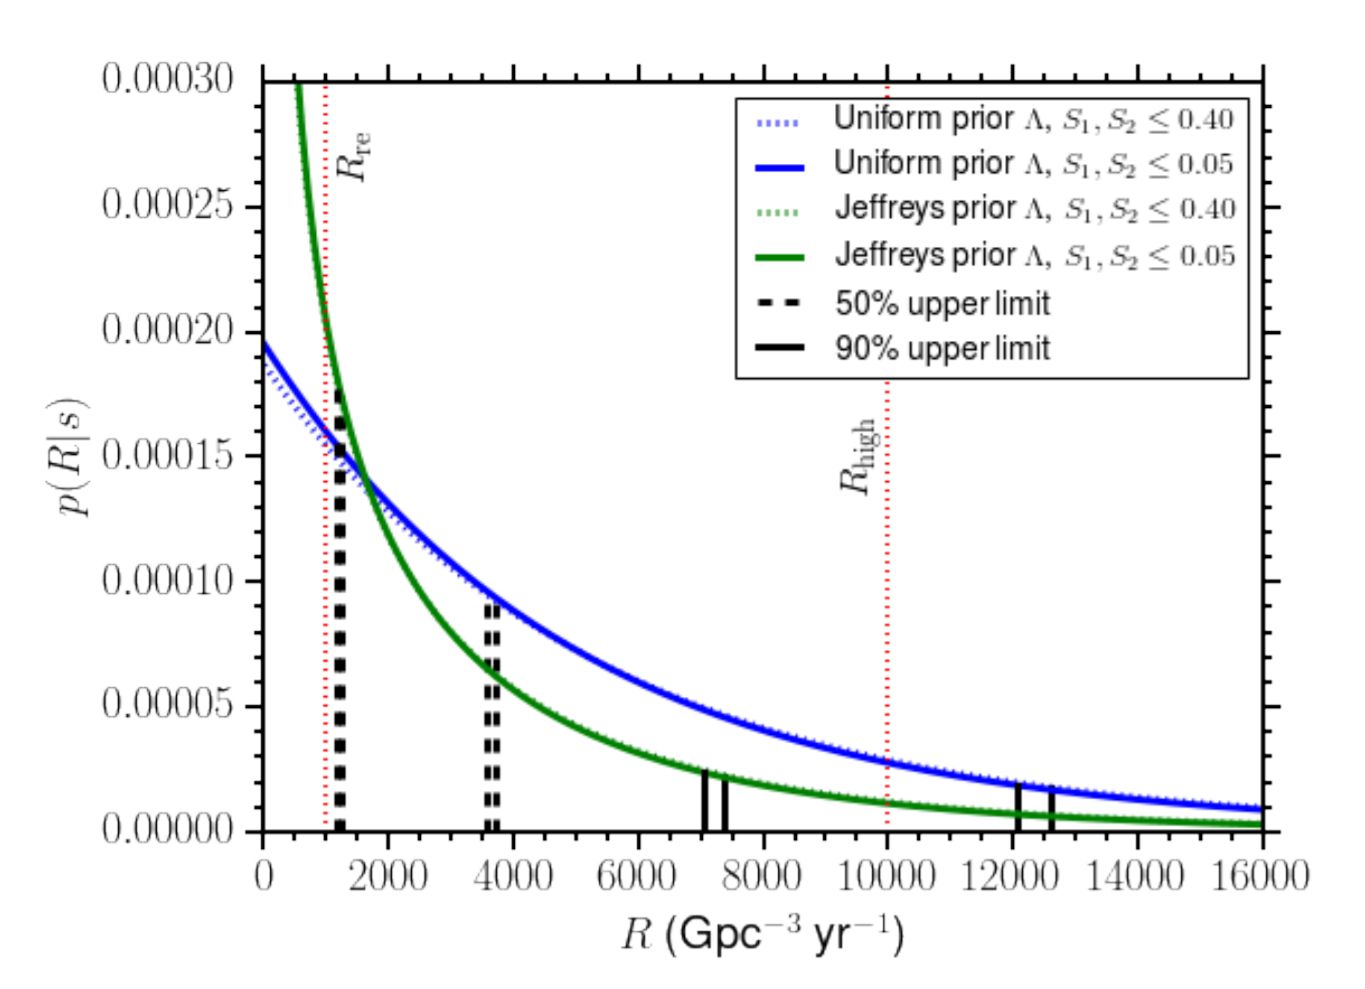
\includegraphics[width=\linewidth]{figs/chapter4/bns_upper_limits_posterior_rates.png}
  \caption{Posterior probability density on the rate of BNS mergers. Blue curves represent a uniform prior on $\Lambda$, while green curves represent a Jeffreys prior on $\Lambda$. The solid (low spin population) and dotted (high spin population) posteriors almost overlap. The vertical dashed and solid lines represent the $50\%$ and $90\%$ credible upper limits respectively for each choice of prior on $\Lambda$. For each pair of vertical lines, the left line is the upper limit for the low spin population and the right line is the upper limit for the high spin population. Also
  shown are the realistic $R_\mathrm{re}$ and high end $R_\mathrm{high}$ of the expected BNS merger rates identified in Ref. (Abadie et al. 2010).}
  \label{fig:bns_upper_limits}
\end{figure}

\begin{figure}
    \centering
    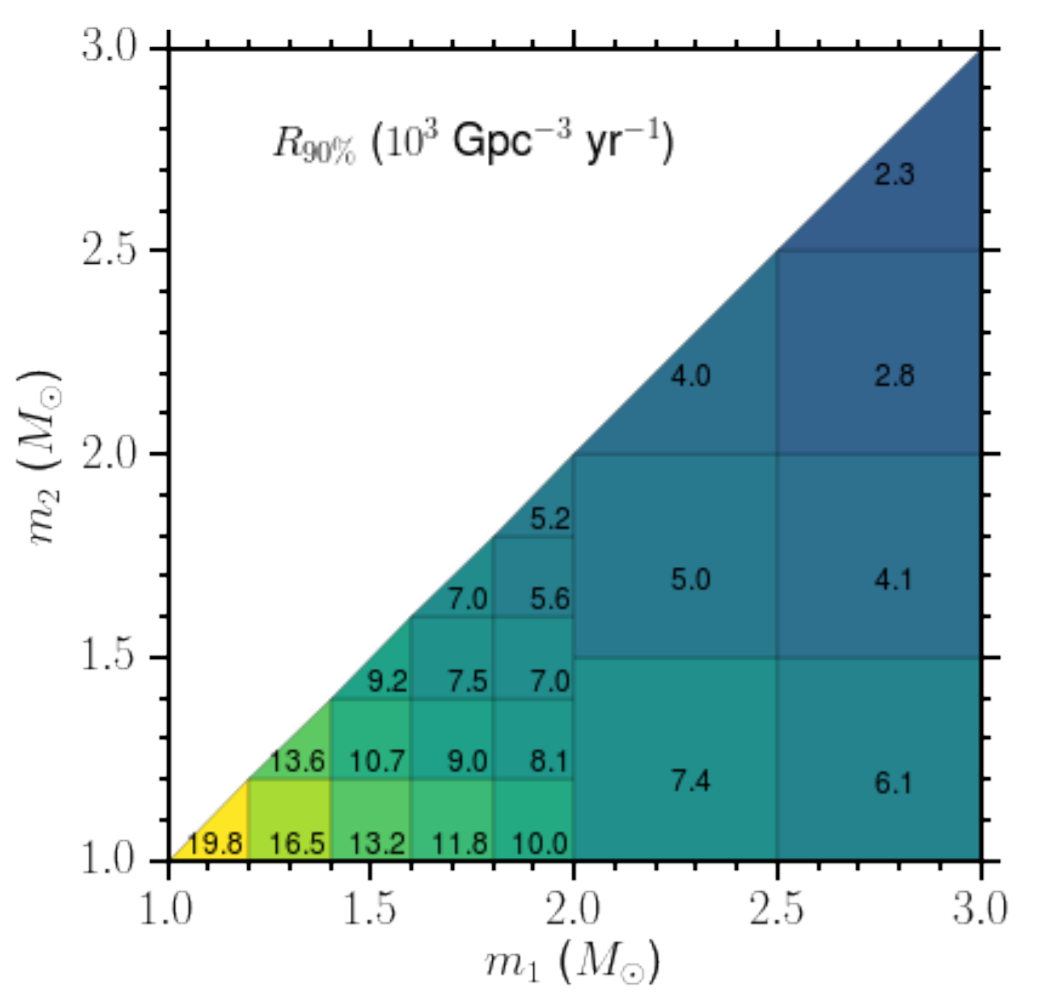
\includegraphics{figs/chapter4/bns_uniform_mass_isotropic_low_spin_rates.png}
    \caption{The $90 \%$ credible upper limit on the BNS merger rate as a function of the two component masses. Here the upper limit for each bin is obtained assuming a BNS population with masses distributed uniformly within the limits of each bin, considering isotropic spin direction and dimensionless spin magnitudes uniformly distributed in $[0,0.05]$.}
    \label{fig:bns_uniform_upper_limits}
\end{figure}

The $90 \%$ posterior probabilty upper limits on the rate of mergers for NSBHs can be summarized in Table~\ref{tbl:nsbh_posteriors}. We found that the search is less sensitive to populations of NSBHs with isotropic spin distributions when compared to (anti-) aligned spin distributions. One factor that contributes to this increased sensitivity to (anti-) aligned spin NSBHs is the fact that the template bank is constructed using (anti-) aligned spin templates and not isotropic-spin distributed templates.

\begin{table}[h!]\label{tbl:nsbh_posteriors}
\centering{}
 \begin{tabular}{||c c c c ||}
 \hline
 NS Mass ($M_\odot$) & BH Mass ($M_\odot$) &  Spin Distribution & $R_{90 \%}$ \, ($Gpc^{-3} \, yr^{-1}$) \\
 \hline\hline
 1.4 & 5 & Isotropic & 3,600 \\ 
 \hline
 1.4 & 5 & Aligned & 3,210 \\
 \hline
 1.4 & 10 & Isotropic & 2,530 \\
 \hline
 1.4 & 10 & Aligned & 1,850 \\
 \hline
 1.4 & 15 & Isotropic & 2,300 \\
 \hline
 1.4 & 15 & Aligned & 1,280 \\
 \hline
\end{tabular}
\caption{The $90\%$ credible upper limit for NSBH systems with isotropic and aligned  spin distributions. The NS spin magnitudes are in the range [0,0.04] and the BH spin magnitudes are in the range [0,1].}
\end{table}


\section{Astrophysical Interpretation and Future Results}
The inferred upper limit estimation on the rate of binary mergers for compact binary mergers involving neutron stars permit us to explore if any population models for the genesis of these binaries can be ruled out by the available data. For BNS populations we compare our posterior rate estimations with $10$ other studies. While for the NSBH populations we compare our posterior rate estimations with $9$ other studies.

For BNS populations we consider the population models from : During the first observing run our upper limit estimations on the rate of BNS mergers were not in conflict with any of the population models considered. It was estimated that assuming estimates of O2 and O3 aLIGO detector sensitivities that continued non-detections of BNS mergers in aLIGO's  second observing run and third observing run that our upper limits could begin to rule out some of the population models considered. Fortunately, however GW170817, a BNS merger event, was discovered in the second observing run.

For NSBH poppulations we consider the population models from:



BNS and NSBH mergers are considered to be possible sources for short-hard gamma ray bursts (). We can also explore a geometrical argument regarding the beaming angle of binary neutron stars and neutron star-black hole binaries if they are assumed to be the progenitors of short-hard gamma ray burst events.

Rate Implications on population Models

Explain short-hard gamma ray bursts...
Assuming that every merger from a BNS or an NSBH produces a gamma ray burst the rate of short-hard gamma ray bursts detected follows from a geometric relationship of the beaming angle of the gamma ray burst jet and the expected rate of mergers of these binaries. The relation can be given as follows:
\begin{equation}\label{eqn:grb_jet_angle}
    R_\mathrm{GRB} = \left[ 1 - cos \left(\theta_\mathrm{jet}\right) \right] R_\mathrm{merger}.
\end{equation}
The relation can be understood as an axially symmetric jet whose solid angle covers a fraction of a unit sphere that envelops the binary. Hence, for some rate of binary mergers, $R_\mathrm{merger}$, a fraction of these mergers will be seen as gamma ray bursts from which we can infer a rate of gamma ray bursts, $R_\mathrm{GRB}$. This fraction is related to the opening angle of the gamma ray jet, $\theta_\mathrm{jet}$. In blank we assumed a rate of gamma ray bursts of $R_{\mathrm{GRB}} = 10^{+20}_{-7} \mathrm{Gpc}^{-3} \mathrm{yr}^{-1}$ from (Nakar et al. 2006; Coward et al. 2012). The inferred beaming angles can then be constructed by using the estimates on $R_\mathrm{merger}$ from this study. The study found that we could infer at $90\%$ confidence that the gamma-ray burst jet angle must be greater than $2.\!\!^\circ3_{-1.1}^{1.7}$ if short-hard gamma ray bursts are exclusively caused by BNS mergers and if each BNS merger produces a short-hard gamma ray burst. This inference comes from the low-spin, Gaussian mass distribution population of BNS. If NSBH mergers from $5 M_\odot$ and $1.4 M_\odot$ with aligned spin distributions are considered as the main progenitors of short-hard gamma ray bursts then the 90$\%$ confidence interval is $\theta^{\mathrm{lower \, limit}}_\mathrm{jet} = 4.\!\!^\circ3_{-1.9}^{+3.1}$.

\subsection{GWTC-1: Inferences from the $1^{\mathrm{st}}$ and $2^{\mathrm{nd}}$ Observing Run}
The LIGO Scientific Collaboration and Virgo Collaboration (LVC) found in [] that from the confident BNS merger, GW170817, that they were able to place a posterior estimate on the rate of BNS mergers in the universe to be, at the $90\%$ credible interval to be between $110 - 3840 \, \mathrm{Gpc}^{-3}\mathrm{yr}^{-1}$, and with no confident NSBH merger detections a $90\%$ confidence upper limit on the rate of NSBH mergers of $610 \, \mathrm{Gpc}^{-3}\mathrm{yr}^{-1}$. Note that the $90^\mathrm{th}$ percentile matches relatively closely with the $50^\mathrm{th}$ percentile estimate for the uniform prior distribution on $\Lambda$ in Fig.~\ref{fig:bns_upper_limits}. The procedure for generating an upper limit on the rates given a detection event is somewhat different from the procedure outlined in this chapter, however the procedure in [] for estimating the upper limit on the rate of NSBH mergers is mostly identical to the procedure outlined in this chapter, with the exception of some changes to the PyCBC offline search pipeline in terms of ranking statistic of candidate triggers.
